% ⚠️ SEM orcidID: um identificador de exemplo e um identificador INVENTADO, e este
% projecto nao inventa identificadores. Se o autor tiver ORCID, acrescenta-se o real.
% ICITS'27 -- 10th International Conference on Information Technology & Systems.
% Cusco, Peru (and online), 27-29 January 2027. Submission 27 September 2026.
% Proceedings: Springer LNNS, indexed in Scopus / WoS / DBLP. Up to 12 pages.
%
% Focus agreed with the supervision: the proposed architecture and the main evaluation
% results, selecting from the dissertation only what serves that purpose.
%
% EVERY NUMBER HERE HAS A SOURCE. `python scripts/check_artigo_numeros.py` fails when a
% figure appears that neither the dissertation nor docs/evaluation/ sustains, and when a
% result the dissertation NARROWED appears here without the same caveat. That gate exists
% because on 2026-09-04 this paper still claimed the aggregate retrieval result the
% dissertation had already disowned.
\documentclass[runningheads]{llncs}

\usepackage[T1]{fontenc}
\usepackage[utf8]{inputenc}
\usepackage{graphicx}
\usepackage{booktabs}
\usepackage{amsmath,amssymb}
\usepackage{tikz}
\usetikzlibrary{arrows.meta, positioning, calc}
\usepackage[hidelinks]{hyperref}

% As figuras do artigo sao as da arvore INGLESA, por ser essa a sua lingua. Enquanto
% as duas arvores partilhavam ficheiros identicos isto nao tinha efeito visivel; deixou
% de ter quando a primeira figura passou a existir em duas linguas.
\graphicspath{{../tese-eng/figures/}}

\begin{document}

\title{Explaining Without Predicting: Statistical Anomaly Detection and Precedent
Retrieval for Verifiable Financial Alerts}

\titlerunning{Explaining Without Predicting}

\author{Henrique J.\,S.\ Santos\inst{1} \and
Lu\'is Gomes\inst{1} \and
Rafael Silva\inst{1}}

\authorrunning{H.\,J.\,S.\ Santos et al.}

\institute{Instituto Superior de Engenharia do Porto (ISEP), Porto, Portugal\\
\email{1180934@isep.ipp.pt}}

\maketitle

\begin{abstract}
Retail investors face a continuous stream of price movements and financial news without
the interpretive tools available to institutions. We present InvestiGator, an
explainable financial alerting system for the US equity market, built exclusively on free
data sources and deployed in continuous operation. The system answers three questions a
retail investor faces when a price moves, and attaches to every alert the evidence that
supports it: whether the movement is unusual for that company, whether its origin lies
with the company or the market, and whether comparable precedents exist and what followed
them. A design constraint runs through the architecture: the system issues no price
forecasts, because a statement about a past event can be checked against the record at the
moment it is read, whereas a forecast can only be assessed after the decision it informs
has been taken. Each component is evaluated against transparent baselines declared in
advance. Volatility-normalised detection fires at a near-constant rate across companies of
very different volatility, with a spread of $0.015$ against $0.344$ for a fixed-threshold
rule, and outperforms two learned detectors under an equivalent causal protocol. Semantic
retrieval beats the sector base rate in all five sectors evaluated and retains its margin
under the temporal constraint the deployed system faces. A supervised triage model
\emph{does not} outperform a volatility-only baseline: added to a per-company lookup table,
the headline text contributes $+0.012$ PR-AUC, an upper bound rather than a usable
quantity. We report that negative result with the same prominence as the positive ones, and
locate it: the information the text carries separates companies and periods, where the
product needed it to separate news items.

\keywords{Explainable AI \and Financial alerting \and Anomaly detection \and
Semantic retrieval \and Retail investors}
\end{abstract}

%======================================================================
\section{Introduction}
%======================================================================

Buying shares has become a low-friction operation. Most American adults now hold equities,
directly or through funds and retirement plans~\cite{gallup2025stock}, in a market whose
capitalisation exceeds 62 trillion US dollars~\cite{sifma2025factbook}. Ease of access has
not extended to interpretation. When a price moves, the retail investor has limited means
of determining what that movement means.

Three concrete questions remain unanswered at the moment an investor observes a price
move. First, \emph{is the movement unusual?} A four per cent change is a rare event for a
low-volatility company and an ordinary day for a volatile one. Second, \emph{does the
movement originate with the company or with the market?} A decline that tracks the index
and an isolated decline are different situations. Third, \emph{are there precedents, and
what followed them?}

Free applications display the percentage change; the few that go further deliver a
generated summary without the evidence behind it. Professional terminals answer all three,
at subscription costs incompatible with this audience. The gap is not one of data
availability, which is ample and free, but of verifiable context built on top of it.

This paper presents InvestiGator, a deployed system that answers the three questions and
exposes the evidence for each answer, and reports the evaluation of its components. As an
Artificial Intelligence Engineering contribution, the work lies not in formulating a new
algorithm but in the selection, integration and critical evaluation of established
techniques until they constitute a functioning, explainable and reproducible system,
including the result that contradicts the initial hypothesis.

\paragraph{A design constraint.} The system produces \emph{no price forecasts}. It gives no
directional indication, issues no buy or sell recommendations and displays no price
targets. This has two justifications. The first is verifiability: a statement about a past
event can be confirmed against the record at the moment it is read, whereas a forecast is
only assessable after the investor's decision has been taken. The second is theoretical:
the semi-strong form of the efficient market hypothesis~\cite{fama1970efficient} makes
systematic anticipation from public information unlikely. This work neither tests that
hypothesis nor relies on it to establish any conclusion.

%======================================================================
\section{Related Work}
%======================================================================

Each component the system uses exists in the literature in isolation. What does not exist
is their combination under a zero-cost constraint, with the evidence delivered to the user
at the moment the claim is made.

\paragraph{Anomaly detection in financial series.} Surveys of anomaly
detection~\cite{chandola2009anomaly} distinguish statistical from learned approaches.
Isolation Forest~\cite{liu2008isolation} and the Local Outlier
Factor~\cite{breunig2000lof} define rarity geometrically and were designed for spaces with
several interacting variables. Financial return series exhibit volatility clustering, the
property that the ARCH and GARCH families formalise~\cite{engle1982arch,bollerslev1986garch}: periods of agitation follow periods of calm. That structure is
temporal rather than geometric, which conditions the comparison reported in
Sect.~\ref{sec:eval}.

\paragraph{Sentence representation and retrieval.} Contextual encoders~\cite{devlin2019bert}
transformed text representation, but their raw sentence embeddings are poorly suited to
similarity search. Sentence-BERT~\cite{reimers2019sbert} adds the \emph{training
objective} that places sentences in a space where distance means similarity, which is the
property retrieval requires. Domain-specific financial encoders exist~\cite{liu2020finbert,huang2023finbert}; the natural assumption that they transfer to this task is tested in
Sect.~\ref{sec:eval} and does not hold.

\paragraph{Event studies and case-based reasoning.} Measuring what followed an event is the
subject of the event-study method~\cite{brown1985daily}, and sensitivity estimation
benefits from shrinkage towards a reference~\cite{vasicek1973beta}. Presenting past cases
rather than a rule is the premise of case-based reasoning~\cite{aamodt1994cbr}. The system
combines the two: it retrieves semantically close cases and reports the price behaviour
\emph{measured} after each, rather than a prediction derived from them.

\paragraph{Explainability and trust.} The literature distinguishes explaining an opaque
model \emph{post hoc}~\cite{ribeiro2016lime,lundberg2017shap} from building a system whose
reasoning is inspectable by construction~\cite{rudin2019stop}. This work takes the second
route, and the reason is one of risk: trust in automated systems fails in both
directions~\cite{lee2004trust}, and the mere presence of an explanation increases
acceptance of incorrect answers~\cite{bansal2021whole}. A generated sentence is an
assertion; a sentence composed from computed objects is an assertion with the evidence
attached, in which every displayed value points back to the measurement that produced it.

%======================================================================
\section{The InvestiGator System}
\label{sec:system}
%======================================================================

Figure~\ref{fig:arch} shows the components and their connections. Sources on the left,
methods in the centre, delivery channels on the right.

\begin{figure}[t]
\centering
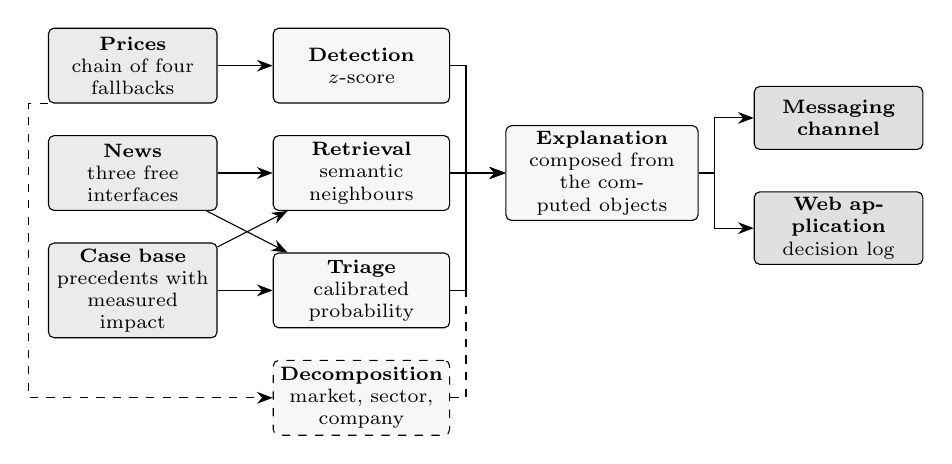
\begin{tikzpicture}[
  font=\scriptsize, >={Stealth[length=2mm]},
  fonte/.style={draw, rounded corners=2pt, align=center, text width=2.0cm,
                minimum height=0.95cm, fill=black!8, inner sep=2pt},
  proc/.style={draw, rounded corners=2pt, align=center, text width=2.1cm,
               minimum height=0.95cm, fill=black!3, inner sep=2pt},
  saida/.style={draw, rounded corners=2pt, align=center, text width=2.0cm,
                minimum height=0.8cm, fill=black!12, inner sep=2pt},
]
  \node[fonte] (p) {\textbf{Prices}\\ chain of four\\ fallbacks};
  \node[fonte, below=4mm of p] (n) {\textbf{News}\\ three free\\ interfaces};
  \node[fonte, below=4mm of n] (h) {\textbf{Case base}\\ precedents with\\ measured impact};

  \node[proc, right=0.7cm of p] (det) {\textbf{Detection}\\ $z$-score};
  \node[proc, right=0.7cm of n] (rec) {\textbf{Retrieval}\\ semantic\\ neighbours};
  \node[proc, right=0.7cm of h] (tri) {\textbf{Triage}\\ calibrated\\ probability};
  \node[proc, dashed, below=4mm of tri] (dec) {\textbf{Decomposition}\\ market, sector,\\ company};

  \node[proc, right=0.7cm of rec, text width=2.3cm] (exp)
    {\textbf{Explanation}\\ composed from\\ the computed objects};

  \node[saida, right=0.7cm of exp, yshift=7mm] (tg) {\textbf{Messaging channel}};
  \node[saida, right=0.7cm of exp, yshift=-7mm] (web) {\textbf{Web application}\\ decision log};

  \draw[->] (p) -- (det); \draw[->] (n) -- (rec); \draw[->] (h) -- (rec);
  \draw[->] (h) -- (tri); \draw[->] (n) -- (tri);
  \draw[->, dashed] (p.south west) -- ++(-0.25,0) |- (dec.west);
  \draw[->] (det.east) -- ++(0.2,0) |- (exp.west);
  \draw[->] (rec) -- (exp);
  \draw[->] (tri.east) -- ++(0.2,0) |- (exp.west);
  \draw[->, dashed] (dec.east) -- ++(0.2,0) |- (exp.west);
  \draw[->] (exp.east) -- ++(0.2,0) |- (tg.west);
  \draw[->] (exp.east) -- ++(0.2,0) |- (web.west);
\end{tikzpicture}
\caption{System components and their connections. Decomposition is dashed because it is
the only component that does not take part in every evaluation: without a price movement
there is nothing to apportion.}
\label{fig:arch}
\end{figure}

\subsection{The Composition Rule}

One construction rule runs through the whole implementation: the text delivered to the user
is \emph{composed} from the objects the components produced, and is not written by a
language model. Each displayed value comes from the object that computed it, so the alert
cannot state a value other than the one the system obtained. Fidelity is therefore a
property of the construction, not the outcome of a subsequent check.

The system does implement a grounded generation layer, in which every sentence must cite an
evidence record and a verifier rejects any sentence whose numbers do not belong to the
records it cites. That layer is \emph{implemented and evaluated but not exposed} in the
deployed product; it is reported separately in Sect.~\ref{sec:eval} for that reason.

\subsection{Detection: What Counts as Unusual}

A movement is unusual relative to the company's own recent behaviour, not to a fixed
percentage. For each trading day $t$, the log return $r_t = \ln(P_t / P_{t-1})$ is compared
with the mean and standard deviation of the preceding window:
\begin{equation}
z_t = \frac{r_t - \mu_{t-1}}{\sigma_{t-1}},
\qquad
\mu_{t-1}, \sigma_{t-1} \text{ over } [t-w,\, t-1].
\label{eq:zscore}
\end{equation}
The day being assessed is \emph{excluded} from the window that defines its own norm.
Without that exclusion the day would contribute to the mean and deviation against which it
is compared, attenuating its own anomaly. The same discipline forbids the use of any
information later than the day assessed, and an automated test enforces it by mutating the
future of an example and requiring the inputs to remain identical while the label changes.

\subsection{Decomposition: Company or Market}

The observed return is apportioned into a market component, a sector component orthogonal
to the market, and a company-specific residual:
\begin{equation}
r = \beta_m\, r_m + \beta_s\, \tilde{r}_s + \varepsilon .
\label{eq:decomp}
\end{equation}
Sensitivities are estimated only on data \emph{prior} to the day being explained, and are
shrunk towards a reference by precision weighting~\cite{vasicek1973beta} rather than
clipped at an arbitrary bound. The distinction is not cosmetic: a clipping rule that falls
back to a unit sensitivity whenever the estimate leaves a fixed range attributes the whole
of an unusual movement to the company precisely on the days when the estimate is least
reliable, which are the days the alert is about.

\subsection{Retrieval: Precedents with Measured Outcomes}

Each headline is encoded into a $384$-dimensional sentence
embedding~\cite{reimers2019sbert}, and precedents are retrieved by cosine similarity from a
case base of $38{,}214$ entries. What distinguishes retrieval here from a similarity search
is that every retrieved case carries the price behaviour \emph{measured} after it, over
$+1$, $+3$ and $+5$ trading days, aligned to the first session on or after the news date.
Precedents are shown individually, with date, similarity and outcome, and never summarised
into an average that could be read as a forecast.

\subsection{Decision Policy}

Communicating every candidate is equivalent to communicating nothing. A channel delivering
fifteen messages a day stops being read, and the system loses the usefulness that justifies
it. Five decision points act in sequence: the headline must name the company; it must be
recent; a precedent must exceed a similarity floor; the triage score must exceed a floor;
and a global budget of five alerts per day must not be exhausted. Over 1--3 September 2026
the system evaluated $743$ distinct headlines from twelve companies and delivered $15$
alerts to eight of them.

That total of fifteen is the ceiling the budget imposes rather than a measurement: the
budget was exhausted on all three days. What the per-company distribution measures is the
ordering \emph{within} that ceiling, which the policy does not fix, since no company holds
a quota of its own.

%======================================================================
\section{Evaluation}
\label{sec:eval}
%======================================================================

Every comparison is against a baseline chosen and declared \emph{before} the measurement,
which is the condition under which a result can come out negative. Each study states the
question, the procedure and the alternative, the result obtained, and what the result does
\emph{not} allow one to conclude.

\subsection{Detection Is Consistent Across Companies}

The primary argument is label-free: a detector that measures rarity relative to each
company's own norm should fire at a comparable rate across companies of very different
volatility. Over three years of daily data for fifteen large-cap US tickers, the spread
between the most and the least flagged company is $0.015$ for the rolling $z$-score against
$0.344$ for a fixed three per cent rule. Against an approximate extreme-move label the
$z$-score reaches $F_1 = 0.516$ against $0.218$ for the fixed rule.

Under an equivalent causal protocol the same method also outperforms two detectors designed
for this task, with $F_1$ of $0.530$ against $0.269$ for the Isolation
Forest~\cite{liu2008isolation} and $0.280$ for the Local Outlier
Factor~\cite{breunig2000lof}. The literature situates that outcome: both learned detectors
define rarity geometrically and were designed for multivariate spaces, whereas the problem
here presents a single return series per company in which the relevant structure is
temporal. When the assumption embedded in a simple method coincides with the actual
structure of the problem, the margin for improving on it is small.

\paragraph{What this does not establish.} The deployed configuration is not the best
measured within its own family: an exponentially weighted estimator reaches $F_1 = 0.664$
and a sixty-day window $0.678$, against $0.516$ in production. The window was kept for
responsiveness and the equally weighted deviation for explainability. Those are decisions,
not results, and the paper reports them as such.

\subsection{Retrieval Beats the Base Rate in Every Sector}

Relevance is approximated by sector membership, a verifiable proxy rather than the property
one would wish to measure, and the query's own company is excluded so that the task cannot
be solved by ticker matching. Over $3{,}714$ real headlines across five sectors, MiniLM
reaches a cross-ticker precision@5 of $0.514$ and the larger MPNet $0.538$, both above the
lexical baseline of $0.346$; recency, at $0.126$, is worse than random.

The aggregate is not, however, the right way to state the result, and we state the weaker
claim the data supports. Almost half the corpus is technology news, which makes available a
strategy that uses no model and does not even read the query: always return technology
headlines. Its precision equals the fraction of technology queries, $0.467$, above the
lexical baseline. That strategy is useless as a product, since it is right on every query in
one sector and wrong in the four others, but its existence shows that the aggregate partly
measures corpus composition. The comparison that survives the objection is made
\emph{within} each sector, where the method exceeds the corresponding reference value in all
five (Fig.~\ref{fig:persector}).

\begin{figure}[t]
\centering

\includegraphics[width=\textwidth]{eval_retrieval_sector_causal.pdf}
\caption{Left, per-sector cross-ticker precision@5 against the sector base rate: the
absolute margin is largest in the most abundant sector, while in the scarce sectors, where
the reference value is near $0.072$, the method reaches several times that value with a
smaller absolute margin. Right, the same measurement under the constraint the deployed
system faces, that a precedent must predate the query: precision falls to $0.513$ and the
base rate to $0.259$, so that the margin over chance moves by $0.008$.}
\label{fig:persector}
\end{figure}

Two checks bound the claim, and the right-hand panel of Fig.~\ref{fig:persector} shows
them. On the multi-year corpus of approximately eighty thousand headlines, precision@5
rises to $0.595$ while the base rate rises in the same proportion: the method neither
degrades nor improves with scale. Imposing the constraint the deployed system actually
faces, that a precedent must predate the query, lowers precision to $0.513$ and the base
rate to $0.259$, moving the margin by $0.008$. The method keeps its advantage
when forced to operate as it does in production.

\paragraph{Theme is not direction.} Agreement between the direction of the query's movement
and that of its precedents is $0.708$ against a chance value of $0.688$. Two headlines can
concern the same subject and the prices move in opposite directions. The consequence for the
product is the decision to present precedents individually, with date and outcome, rather
than reducing them to an average that could be read as a forecast.

\subsection{The Negative Result: Text Does Not Beat Volatility}

The triage task is to decide, before delivery, which headlines justify interrupting the
reader. We built a dataset of $79{,}753$ examples from the public FNSPID
corpus~\cite{dong2024fnspid} and price series, with a single-day temporal split and an
embargo, and trained six families. Table~\ref{tab:triage} reports them.

\begin{table}[t]
\centering
\caption{Triage, PR-AUC on the held-out test block (prevalence $0.378$). The baseline
declared in advance was the volatility-only model.}
\label{tab:triage}
\begin{tabular}{lcc}
\toprule
Model & PR-AUC & Brier \\
\midrule
Volatility only (baseline) & $\mathbf{0.542}$ & $0.218$ \\
Company and day context & $0.538$ & $0.224$ \\
Context and headline text & $0.496$ & $0.229$ \\
Gradient boosting & $0.469$ & $0.228$ \\
Headline text only & $0.439$ & $0.240$ \\
Always alert (floor) & $0.378$ & $0.622$ \\
\bottomrule
\end{tabular}
\end{table}

No variant incorporating the headline text outperforms the volatility-only baseline. The
result survives three checks. The first repeats the comparison granting the text the best
available conditions, with tuned regularisation, a PCA-reduced text block and a
finance-domain encoder, and raises its best value to $0.533$ without reaching the baseline.
The second resamples by groups formed of company and day, and keeps the interval excluding
zero. The third repeats the measurement for nine alternative combinations of label
threshold and horizon, and volatility matches or exceeds the text model in all nine.

\paragraph{The domain encoder is the weakest of all.} The finance-specific encoder reaches
$0.420$, the lowest value among the models evaluated. The artefact assessed is the public
checkpoint \texttt{ProsusAI/finbert}, applied by mean-pooling its vectors, which is the way
to use it without further training. It is an encoder tuned for sentiment classification and
not for placing sentences in a space where distance means similarity, and it is precisely
that training objective that Sentence-BERT adds~\cite{reimers2019sbert}. The measurement
establishes that this domain model, used in this way, performs worse than a general model
trained for similarity; it does not establish that domain knowledge is irrelevant to the
task.

\subsection{Locating the Negative Result}

Placing representations side by side answers which of them is better. The question with
more use to whoever builds a system is different: does the text add to what is already
known? Measured against a per-company lookup table, which contains everything the model
knows about the company and nothing about the news item, the answer is affirmative: the
headline adds $+0.012$ PR-AUC, with an interval between $+0.004$ and $+0.020$ that excludes
zero. It is the only occasion on which a text representation shows a detectable increment
in this task.

The value falls below the $0.02$ threshold fixed before the measurements, and that
threshold applies in both directions. What is established is an \emph{upper bound} on the
effect of the text, not a quantity the system can use. Three further measurements prevent
this increment from reopening the verdict: the sum does not exceed volatility alone; the
increment does not survive the metric that describes the product, since precision within the
five-alert budget remains at $0.662$ with and without text; and the ability to separate news
items from the same company remains at chance level.

What these measurements add to the negative answer is not a caveat but a \emph{location}:
the information the text carries separates companies and periods, where the product needed
it to separate news items.

\paragraph{An engineering consequence.} A per-company lookup table of thirteen constants,
containing no information from any headline, reaches $0.534$ against $0.538$ for the
deployed variant, and the same precision within budget. The deployed model \emph{is}, in
effect, a lookup table. That finding is what led to the policy change reported next.

\subsection{The System in Operation}

The system has run continuously on free infrastructure, monitoring twelve companies. Over
the periods documented it delivered $367$ messages, between 9 July and 13 August 2026, and
recorded $36{,}925$ triage decisions over a wider window, while the precedent base
accumulated $38{,}214$ cases with measured impact.

\paragraph{A measured policy change.} Once the triage model was found to be a lookup table,
it was changed from a veto into a ranking, under a global daily budget. The effect was
measured, with a control. In news alerts, which the budget governs, concentration in the
three most alerted companies falls from $0.713$ to $0.480$, with the interval of the
difference excluding zero, and the number of companies reaching an alert rises from seven to
nine of twelve. Price-movement alerts cross the same period, the same companies and the same
conditions, and the budget does \emph{not} count them: in that series concentration moves
from $0.449$ to $0.485$, with the interval containing zero. The governed quantity moved and
the ungoverned one did not.

\paragraph{Grounded generation, measured separately.} For the layer that is implemented but
not exposed, two quantities are measured because they answer different questions. An
adversarial corpus of $23$ attacks, each of which must be rejected, measures the guard:
$23/23$ are blocked. A set of $8$ faithful control sentences, each of which must pass,
measures whether the guard is merely refusing everything: $8/8$ are admitted. The second is
the load-bearing figure, since a guard that rejected all text would score perfectly on the
first.

%======================================================================
\section{Discussion and Limitations}
%======================================================================

\paragraph{No controlled user study.} This is the heaviest gap. The system rests on the
hypothesis that an explanation accompanied by its evidence leads a non-specialist to a
better decision, and that hypothesis has not been submitted to an experimental design. The
protocol exists and has not been executed. What does exist is feedback collected in a real
context: readers of the public channel classify the alerts they receive, under analysis
rules fixed before the first vote. That feedback is observational: participation is
self-selected, no group received the price change without the accompanying explanation, and
the channel is public, so it is not known whether respondents belong to the audience this
work assumes. The founding hypothesis concerns a better decision, which is a different
quantity, and it remains untested.

\paragraph{Latency is bounded by the sources, not by the cycle.} Between publication and
detection the median is $353$ minutes, and between detection and delivery it is five seconds,
with a ninetieth percentile of sixteen.
The time is entirely in discovery, and shortening the polling cycle did not reduce it: free
company-news interfaces are not real-time channels, and the most recent headline in a feed
is not the most recent \emph{relevant} one. The system observes, by construction,
information that is no longer new. That condition aggravates rather than attenuates the
expectation behind the negative result of Sect.~\ref{sec:eval}.

\paragraph{Labels are verifiable approximations.} Sector membership approximates relevance;
a return threshold approximates materiality; a percentile approximates rarity. Each is
verifiable and none is the property one would wish to measure. Closing that distance
requires a human-annotated sample, which does not exist.

\paragraph{Survivorship and coverage.} The companies were selected in 2026 and evaluated
over the past, so they survived by construction. News coverage is incomplete and uneven:
at least one headline was captured on $88.5\%$ of unusual days, which is an upper bound,
since it asks whether \emph{a} story existed and not whether it was the right one.

%======================================================================
\section{Conclusion}
%======================================================================

InvestiGator shows that useful financial alerting for retail investors can be transparent
and reproducible at once: a volatility-normalised detector that explains every flag, a
retrieval engine that returns analogous precedents and reports their \emph{measured}
outcome as evidence rather than prediction, a decomposition that separates the company from
the market, and a calibrated triage model that honestly fails to beat a volatility-only
baseline with text.

The most transferable observation is that last one, and it concerns evaluation rather than
modelling. A component evaluated in isolation, over the distribution of its training set,
and deployed behind filters that change that distribution, has not been evaluated on the
distribution it will see. The metric was correct and the question it asked was not the one
the product needed: PR-AUC over a full test set is dominated by variation \emph{between}
companies, whereas the product required separation \emph{within} a company on a given day.
Detecting that required comparing the deployed model against a lookup table of thirteen
constants, which is a comparison worth making before concluding that a learned component
earns its place.

Future work is a market-adjusted impact-magnitude study over the multi-year precedents, the
controlled user study whose protocol is already prepared, an annotated sample that would
anchor all three labels at once, and closing the text gap with richer input than headlines.

\subsubsection*{Reproducibility.} All results are produced by versioned scripts over frozen
artefacts, with fixed seeds. The trained model, its calibration and the evaluation outputs
are kept as versioned artefacts, and each figure in this paper is regenerated by the script
that produced the corresponding measurement.

\subsubsection*{Acknowledgements.} The authors thank the readers of the public channel who
classify the alerts they receive.

\begin{thebibliography}{99}
\bibitem{gallup2025stock} Gallup: What Percentage of Americans Own Stock? (2025)
\bibitem{sifma2025factbook} SIFMA: Capital Markets Fact Book. Securities Industry and
Financial Markets Association (2025)
\bibitem{fama1970efficient} Fama, E.F.: Efficient capital markets: a review of theory and
empirical work. J. Finance \textbf{25}(2), 383--417 (1970)
\bibitem{chandola2009anomaly} Chandola, V., Banerjee, A., Kumar, V.: Anomaly detection: a
survey. ACM Comput. Surv. \textbf{41}(3), 1--58 (2009)
\bibitem{liu2008isolation} Liu, F.T., Ting, K.M., Zhou, Z.-H.: Isolation forest. In: ICDM,
pp.\ 413--422 (2008)
\bibitem{breunig2000lof} Breunig, M.M., Kriegel, H.-P., Ng, R.T., Sander, J.: LOF:
identifying density-based local outliers. In: SIGMOD, pp.\ 93--104 (2000)
\bibitem{engle1982arch} Engle, R.F.: Autoregressive conditional heteroscedasticity with
estimates of the variance of United Kingdom inflation. Econometrica \textbf{50}(4),
987--1007 (1982)
\bibitem{bollerslev1986garch} Bollerslev, T.: Generalized autoregressive conditional
heteroskedasticity. J. Econom. \textbf{31}(3), 307--327 (1986)
\bibitem{devlin2019bert} Devlin, J., Chang, M.-W., Lee, K., Toutanova, K.: BERT:
pre-training of deep bidirectional transformers for language understanding. In: NAACL,
pp.\ 4171--4186 (2019)
\bibitem{reimers2019sbert} Reimers, N., Gurevych, I.: Sentence-BERT: sentence embeddings
using Siamese BERT-networks. In: EMNLP-IJCNLP, pp.\ 3982--3992 (2019)
\bibitem{liu2020finbert} Liu, Z., Huang, D., Huang, K., Li, Z., Zhao, J.: FinBERT: a
pre-trained financial language representation model for financial text mining. In: IJCAI,
pp.\ 4513--4519 (2020)
\bibitem{huang2023finbert} Huang, A.H., Wang, H., Yang, Y.: FinBERT: a large language model
for extracting information from financial text. Contemp. Account. Res. \textbf{40}(2),
806--841 (2023)
\bibitem{brown1985daily} Brown, S.J., Warner, J.B.: Using daily stock returns: the case of
event studies. J. Financ. Econ. \textbf{14}(1), 3--31 (1985)
\bibitem{vasicek1973beta} Vasicek, O.A.: A note on using cross-sectional information in
Bayesian estimation of security betas. J. Finance \textbf{28}(5), 1233--1239 (1973)
\bibitem{aamodt1994cbr} Aamodt, A., Plaza, E.: Case-based reasoning: foundational issues,
methodological variations, and system approaches. AI Commun. \textbf{7}(1), 39--59 (1994)
\bibitem{ribeiro2016lime} Ribeiro, M.T., Singh, S., Guestrin, C.: ``Why should I trust
you?'': explaining the predictions of any classifier. In: KDD, pp.\ 1135--1144 (2016)
\bibitem{lundberg2017shap} Lundberg, S.M., Lee, S.-I.: A unified approach to interpreting
model predictions. In: NIPS, pp.\ 4765--4774 (2017)
\bibitem{rudin2019stop} Rudin, C.: Stop explaining black box machine learning models for
high stakes decisions and use interpretable models instead. Nat. Mach. Intell.
\textbf{1}(5), 206--215 (2019)
\bibitem{lee2004trust} Lee, J.D., See, K.A.: Trust in automation: designing for appropriate
reliance. Hum. Factors \textbf{46}(1), 50--80 (2004)
\bibitem{bansal2021whole} Bansal, G., Wu, T., Zhou, J., Fok, R., Nushi, B., Kamar, E.,
Ribeiro, M.T., Weld, D.S.: Does the whole exceed its parts? The effect of AI explanations on
complementary team performance. In: CHI, pp.\ 1--16 (2021)
\bibitem{dong2024fnspid} Dong, Z., Fan, X., Peng, Z.: FNSPID: a comprehensive financial news
dataset in time series. In: KDD, pp.\ 4918--4927 (2024)
\end{thebibliography}

\end{document}
